\newpage
\section{XToolKit}
\markright{\arabic{section}. XToolKit}

XToolKit is the highest level X window interface to facilitate composing
GUI (Graphical User Interface) by using GUI components such as
buttons, pulldown menus, textWindows, etc., as building blocks.
The major differences from the Xlib classes are,
the XToolKit invokes user-supplied interaction routines
corresponding to the Xevents sent from the Xserver,
and provides consistent appearance of those interaction-oriented
window parts.
Classes consisting the XToolKit has the following inheritance structure.
\begin{verbatim}
          xwindow
               panel
                    menubar-panel
                    menu-panel
                    filepanel
                    textviewpanel
                    confirmpanel
               panel-item
                    button-item
                         menu-button-item
                         bitmap-button-item
                    text-item
                    slider-item
                    choice-item
                    joystick-item
               canvas
               textwindow
                    buffertextwindow
                         scrolltextwindow
                    textedit
               scroll-bar
                    horizontal-scroll-bar
\end{verbatim}

Just below the xwindow class are the five basic XToolKit classes:
{\tt panel}, {\tt panel-item},
{\tt canvas}, {\tt textWindow} and {\tt scroll-bar}.
{\tt Menubar-panel} and {\tt menu-panel} are defined under the {\tt panel}.
A basic strategy to build a new application window and to make
it run upon events is the following:
\begin{enumerate}
\item{\bf define an application class} An application window class should be
defined as a subclass of {\bf panel} that has the capability to lay out
XToolKit components.
\item{\bf define event handlers} In the application class, event handlers
that are called upon when buttons are pressed or menu items are selected
are defined. An event handler ought to be defined as a method 
with panel-item specific arguments.
\item{\bf define subpanels} If you use a {\tt menubar-panel}, it is placed at the
top of the application window, therefore it should be created first
by {\tt :create-menubar}. Similarly {\tt menu-panel}s needs to be
defined before the {\tt menu-button-item}s to which {\tt menu-panel}s
are associated.
\item{\bf create panel-items} Panel-items such as {\tt button-item},
{\tt text-item}, {\tt slider-item}, etc., can be created
by {\tt (send-super :create-item {\em class label object method})}.
Event handlers defined above are connected to each panel-item.
These initialization procedures should be defined in the {\tt :create}
method of the application window class.
Do not forget to define {\tt quit} button to make the event
dispatcher terminate whenever needed.
Any {\tt textWindow} and {\tt canvas} can also be placed in the application
window via the {\tt :locate-item} method.
\item{\bf create the entire window} Sending the {\tt :create} message to
the application class creates
the application window with its XToolKit components properly placed 
in the window.
%If you do not like the default placement, add {\tt :x} and {\tt :y}
%parameters at the creation of each component.
\item{\bf run the event dispatcher} In order to receive events from the
Xserver and delivers them to the corresponding xwindow,
run {\tt window-main-loop}.
On Solaris2, {\tt window-main-thread}, which delivers events in a
different thread, is available.
{\tt Window-main-thread} keeps the toplevel interaction alive.
Do not run more than one {\tt window-main-thread}.
\end{enumerate}

\subsection{X Event}

In the current implementation, 
an event structure is received in a fixed event buffer (an integer-vector
of 25 elements)
and the same buffer is reused on all events.
The event structure has to be copied when more than one events need to
be referenced at the same time.

{\tt Window-main-loop} is the function which captures all events sent
from the X server and delivers them to each window where the event happened.

\begin{refdesc}

\vardesc{event}{a 25-element integer-vector holding the most recent
event structure.}

\funcdesc{next-event}{}{
stores the event structure in {\tt event} and returns it
if there is at least one pending event,
NIL if there is no pending event.}

\funcdesc{event-type}{event}{
returns the keyword symbol representing the event-type in the {\em event}
structure. The event-type keywords are:
{\tt :KeyPress} (2),
{\tt :KeyRelease} (3),
{\tt :ButtonPress} (4),
{\tt :ButtonRelease} (5),
{\tt :MotionNotify} (6),
{\tt :EnterNotify} (7),
{\tt :LeaveNotify} (8),
{\tt :FocusIn} (9),
{\tt :FocusOut} (0),
{\tt :KeymapNotify} (1),
{\tt :Expose} (12),
{\tt :GraphicsExpose} (13),
{\tt :NoExpose} (14),
{\tt :VisibilityNotify} (15),
{\tt :CreateNotify} (16),
{\tt :DestroyNotify} (17),
{\tt :UnmapNotify} (18),
{\tt :MapNotify} (19),
{\tt :MapRequest} (20),
{\tt :ConfigureNotify} (22),
{\tt :ConfigureRequest} (23),
{\tt :GravityNotify} (24),
{\tt :ResizeRequest} (25),
{\tt :CirculateNotify} (26),
{\tt :CirculateRequest} (27),
{\tt :PropertyNotify} (28),
{\tt :SelectionClear} (29),
{\tt :SelectionRequest} (30),
{\tt :SelectionNotify} (31),
{\tt :ColormapNotify} (32),
{\tt :ClientMessage} (33),
{\tt :MappingNotify} (34),
{\tt :LASTEvent} (35).}

\funcdesc{event-window}{event}{
returns the window object where the {\em event} occurred.}

\funcdesc{event-x}{event}{extracts the {\em x} coordinate,
(i.e., the horizontal position of the mouse pointer relatively in the window)
out of the {\em event}.}
\funcdesc{event-y}{event}{extracts the {\em x} coordinate,
(i.e., the vertical position of the mouse pointer relatively in the window)
out of the {\em event}.}
\funcdesc{event-width}{event}{
returns the eighth element of the {\em event} structure
which represents the width parameter at the {\tt :configureNotify} event.}
\funcdesc{event-height}{event}{
returns the ninth element of the {\em event} structure
which represents the height parameter at the {\tt :configureNotify} event.}
\funcdesc{event-state}{event}{
returns a list of keywords representing the mouse button 
and modifier key state.
Keywords are: {\tt :shift, :control, :meta, :left, :middle} and {\tt :right}.
For example, if left mouse button is pressed while shift key is down,
{\tt (:shift :left)} is returned.}
\funcdesc{display-events}{}{displays all xwindow events captured by
{\tt x:nextevent}. Control-C is the only way to terminate this function.}

\macrodesc{window-main-loop}{\&rest forms}{
receives Xevents and delivers them to window objects where the event
occurred.
According to the event-type, methods in the window's class named 
{\tt :KeyPress, :KeyRelease, :ButtonPress,
:ButtonRelease, :MotionNotify,
:EnterNotify, :LeaveNotify} and {\tt :ConfigureNotify} 
are invoked with {\em event} as the argument.
If {\em forms} is given,
evaluates them each time event arrival is checked.}

\funcdesc{window-main-thread}{}{
Do the same thing as {\tt window-main-loop} in a different thread.
{\tt Window-main-thread} is only available on Solaris2.
{\tt Window-main-thread} installs an error handler which
does not enter a read-eval-print loop.
After printing the error information, the event
processing continues.}

\end{refdesc}

\subsection{Panel}

\begin{refdesc}
\classdesc{panel}{xwindow}
{(pos items fontid\\
\>rows columns	;total number of rows and columns\\
\>next-x next-y\\
\>item-width item-height)}{
Panel is a xwindow with the capability to lay out panel-items or any
xwindows including other panel objects.
A panel object supplies the default font for every panel-item
created in the panel.
Application windows should be defined as subclasses of the {\tt Panel}.}

\longdescription{:create}{\&rest args \= \&key \= ((:item-height iheight) 30)
((:item-width iwidth) 50)
\` [method]\\
\>\> (font font-lucidasans-bold-12)  ((:background color) *bisque1*) \\
\> \&allow-other-keys)}{creates and initializes a panel.
Since superclass's {\tt :create} is invoked,
all creation parameters for {\bf xwindow}, such as {\em width, height, 
border-width}, etc., are allowed.
{\em Item-height} and {item-width} give the minimum height and width
for each panel-item.}

\methoddesc{:items}{}{returns the list of all items associated.}
\methoddesc{:locate-item}{item \&optional x y}{
{\em Item} is any xwindow object, normally a panel-item.
If {\em x} and {\em y} are given, the item is located there.
Otherwise, {\em item} is located adjacent to the most recently located item.
Items are located from top to bottom, from left to right,
as shown in {\bf Fig.} \ref{panellayout}.
{\tt :Locate-item} also adds {\em item} in the {\em items} and {\em subwindows}
 list, and makes it visible by sending {\tt :map}.}

\begin{figure}
\begin{center}
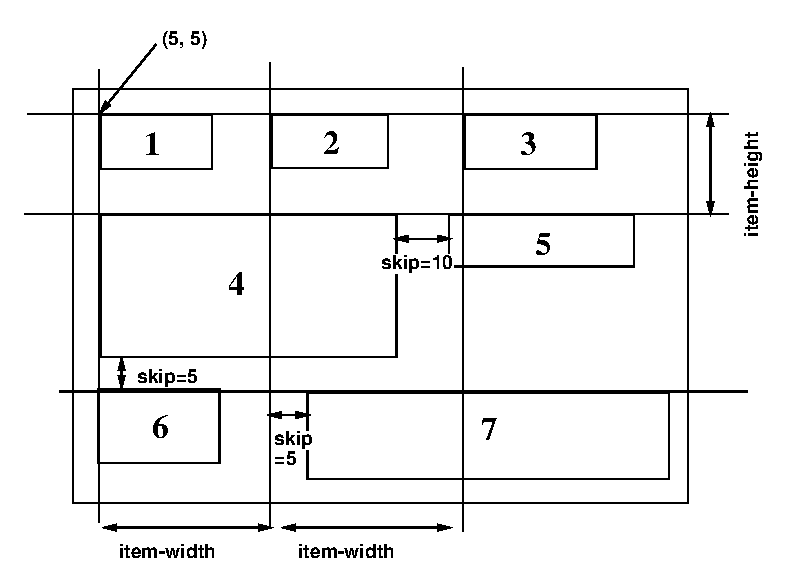
\includegraphics[height=7cm]{fig/panellayout.ps}
%\epsfile{file=fig/panellayout.ps,height=7cm}
%\mbox{
%\epsfysize=7cm
%\epsfbox{fig/panellayout.ps}
%}
\end{center}
\caption{Item lay-out in panel\label{panellayout}}
\end{figure}

\longdescription{:create-item}{klass label receiver method \= \&rest args
\` [method]\\
\> \&key ((font fontid)\\
\> \&allow-other-keys)}{
creates an instance of the panel-item class specified by {\em klass}
(i.e., {\tt button-item,  menu-button-item, slider-item, joystick-item}, etc.),
and place the item in the panel using {\tt :locate-item}.
{\em Args} are passed to {\tt klass}'s {\tt :create} method.
{\em Label} is the identification string drawn in the panel item.
{\em Receiver} and {\em method} specify the event handler called upon
the corresponding event.}

\methoddesc{:delete-items}{}{delete all panel-items.}
\longdescription{:create-menubar}{ \= \&rest args \`[method]\\
\> \&key (font fontid)\\
\> \&allow-other-keys}{
creates a {\em menubar-panel} and  locates it at the top of the panel.}
\end{refdesc}

The following methods are provided to avoid "subclass's responsibility"
warning message when events are sent to panels without event handlers.
User applications should override these methods.

\begin{refdesc}
\methoddesc{:quit}{\&rest a}{
throws {\tt :window-main-loop} and terminates event processing.}
\methoddesc{:KeyPress}{event}{returns NIL.}
\methoddesc{:KeyRelease}{event}{returns NIL.}
\methoddesc{:ButtonPress}{event}{returns NIL.}
\methoddesc{:ButtonRelease}{event}{returns NIL.}
\methoddesc{:MotionNotify}{event}{returns NIL.}
\methoddesc{:EnterNotify}{event}{returns NIL.}
\methoddesc{:LeaveNotify}{event}{returns NIL.}
\end{refdesc}

\subsubsection{Subpanels (menu-panel and menubar-panel)}

\begin{refdesc}
% menu-panel
\classdesc{menu-panel}{panel}{
 (items item-dots item-height\\
                \>charwidth charheight\\
                \>height-offset\\
                \>highlight-item\\
                \>color-pixels\\
                \>active-color)
}{
{\tt Menu-panel} is a kind of panel that can locate only 
{\tt button-item}s and/or {\tt bitmap-button-item}s.
Unlike {\tt panel}, however, {\tt menu-panel} is normally invisible
and is exposed when the {\tt button-item} to which the {\tt menu-panel} is
associated is pressed.
If a {\tt menu-panel} is made always visible, it becomes a pinned menu.
The response of each button-item to mouse events is slightly different from
button-items in other panels,
as the mouse button has been pressed somewhere outside the button-item.
Creation of a {\tt menu-panel} should follow the order described below:
\begin{enumerate}
\item create a menu-panel by {\tt (instance menu-panel :create)}.
\item create button-items or/and bitmap-button-items and locate them in the
menu-panel by {\tt (send aMenuPanel :create-item button-item "BTN" obj meth)}.
\item create a menu-button-item in another panel and associate the menu-panel
with the menu-button-item by {\tt (instance menu-button-item :create
"Option" obj meth :menu-window aMenuPanel)}.
\end{enumerate}
}


\longdescription{:create}{\&rest args \= \&key\= (items) (border-width 0)
   (font font-courb12)
\` [method]\\
\>\> (width 100) (height-offset 15) (color *bisque1*)
                      (active *bisque2*) \\
           \>\&allow-other-keys) 
  }{
create a menu-panel window. The size of the window is expanded each time
new menu-item is added.}

\methoddesc{:create-item}{class label receiver method  \&rest mesg}{
adds a menu item in this menu-panel window and attatches
the corresponding action. 
The {\em receiver} objects receives {\em mesg}
when the mouse button is released on the item.}

% \methoddesc{:popup}{x y \&optional (offset 20)}{
% pops up the menu at the position (x,y) specified on the root window.}
% \methoddesc{:buttonPress}{event}{
% maps the menu-panel  and makes it visible.}
%\methoddesc{:buttonRelease}{event}{
%perform a method coresdonding toa selected item and unmap the menu window.
%}

\classdesc{menubar-panel}{panel}{}{
{\tt Menubar-panel} is a subpanel always located at the top of the parent 
panel. A menubar-panel resembles with the Macintosh desktop's menubar
which lets out several pull-down menus.
Panel-items placed in the menubar should be {\tt menu-button-item}s.
A menubar-panel is created by the panel's {\tt :create-menubar} method.}

\end{refdesc}

\subsubsection{File Panel}
The FilePanel is an application window for the interactive  manipulation
of files and directories.
Using {\tt cd} and {\tt go-up} buttons, any directory can be visited
and files contained in the directory are displayed in the {\tt ScrollTextWindow}
below.
Text files can be displayed in different windows (textViewPanel).
Files can also be printed, removed, and compiled by simply cliking buttons.
When a file is printed, {\tt a2ps {\em file} | lpr} commands are executed
in a forked process.

\begin{figure}
\begin{center}
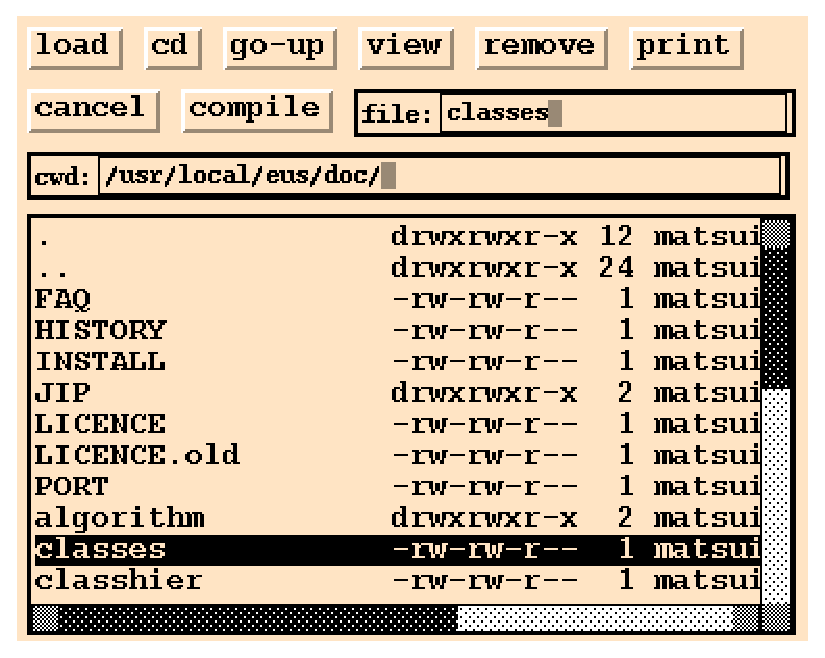
\includegraphics[height=7.5cm]{fig/filepanel.ps}
%\epsfile{file=fig/filepanel.ps,height=7.5cm}
%\mbox{
%\epsfysize=7.5cm
%\epsfbox{fig/filepanel.ps}
%}
\end{center}
\caption{FilePanel window}
\end{figure}

\subsubsection{Text View Panel}

TextViewPanel is an application window class to display text files
(Fig. \ref{textviewpanel}).
The program text is shown to demonstrate how 
one of the simplest application windows is described.
In the {\tt :create} method, the quit button and find button,
and a text-item to feed the string to be searched for in the file
are created.
The view-window is a ScrollTextWindow that displays the file
with the vertical and horizontal scroll-bars.
The TextViewPanel captures {\tt :ConfigureNotify} event
to resize the view-window when the outermost title window is resized
by the window manager.

\begin{figure}
\begin{center}
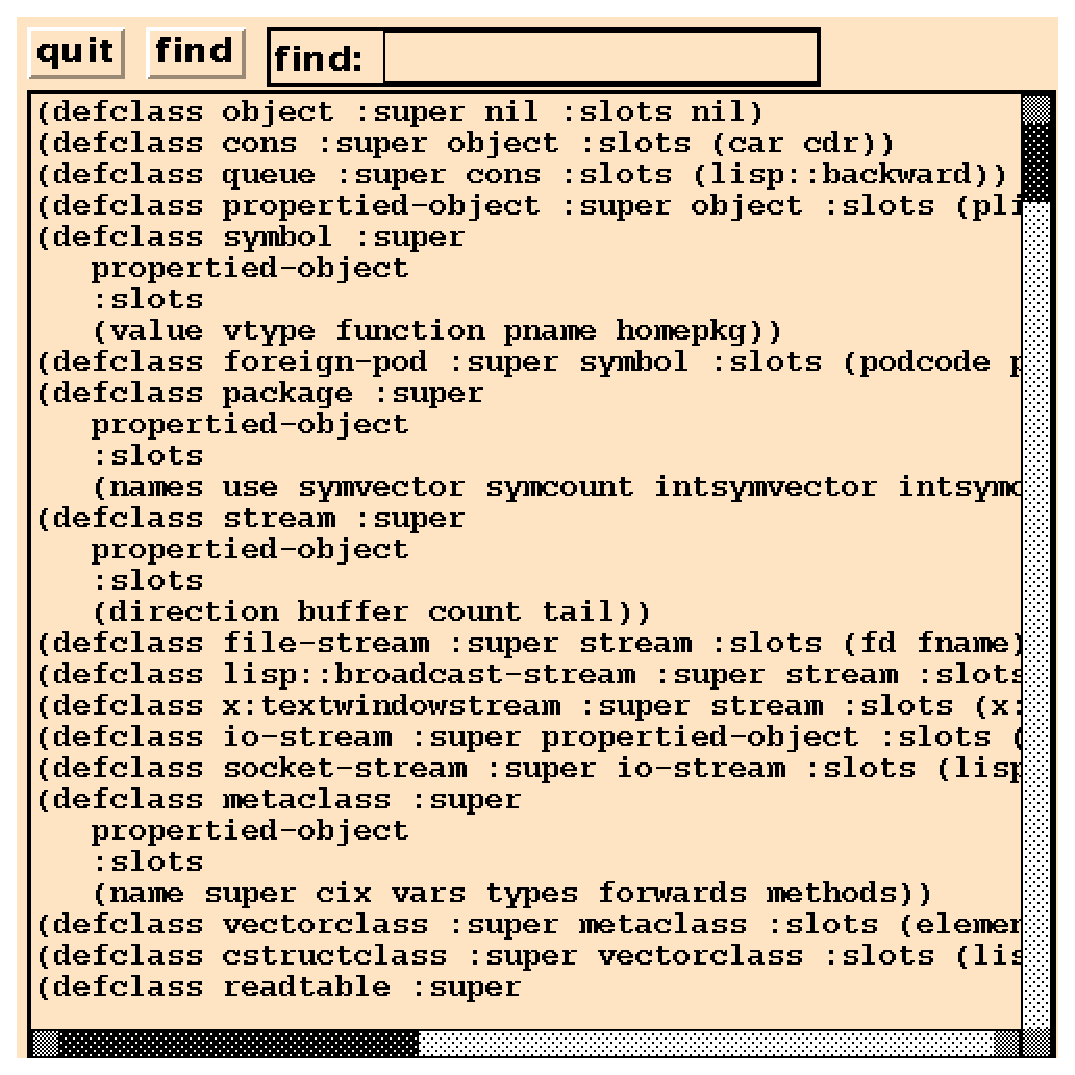
\includegraphics[height=7cm]{fig/textviewpanel.ps}
%\epsfile{file=fig/textviewpanel.ps,height=7cm}
%\mbox{
%\epsfysize=7cm
%\epsfbox{fig/textviewpanel.ps}
%}
\end{center}
\caption{TextViewPanel window\label{textviewpanel}}
\end{figure}

\begin{verbatim}
(defclass TextViewPanel :super panel
        :slots (quit-button find-button find-text view-window))

(defmethod TextViewPanel
 (:create (file &rest args &key (width 400) &allow-other-keys)
    (send-super* :create :width width args)
    (setq quit-button
          (send self :create-item panel-button "quit" self :quit))
    (setq find-button
          (send self :create-item panel-button "find" self :find))
    (setq find-text
          (send self :create-item text-item "find: " self :find))
    (setq view-window
            (send self :locate-item
                (instance ScrollTextWindow :create
                   :width (setq width (- (send self :width) 10))
                   :height (- (setq height (send self :height)) 38)
                   :scroll-bar t :horizontal-scroll-bar t
                   :map nil      :parent self)))
    (send view-window :read-file file))
 (:quit (event)  (send self :destroy))
 (:find (event)
    (let ((findstr (send find-text :value)) (found)
          (nlines (send view-window :nlines)))
        (do ((i 0 (1+ i)))
            ((or (>= i nlines) found))
           (if (substringp findstr (send view-window :line i)) (setq found i)))
        (when found
           (send view-window :display-selection found)
           (send view-window :locate found))))
 (:resize (w h)
    (setq width w height h)
    (send view-window :resize (- w 10) (- h 38)))
 (:configureNotify (event)
   (let ((newwidth (send self :width))
         (newheight (send self :height)))
        (when (or (/= newwidth width) (/= newheight height))
          (send self :resize newwidth newheight)))  ) )
\end{verbatim}

\subsection{Panel Items}
\begin{refdesc}
\classdesc{panel-item}{xwindow}
{(pos notify-object notify-method\\
\>fontid label labeldots)}{
{\bf Panel-item} is an abstract class for all kinds of panel-item windows
to invoke {\em notify-object}'s  {\em notify-method} when item-specific
event occurs.
}

\methoddesc{:notify}{\&rest args}{
invokes {\em notify-object}'s  {\em notify-method}.
Responsive events and arguments passed to {\em notify-method}
are item specific:
\begin{description}
\item [button-item] The button is pressed and released
in the same button-item;
the argument is the button-item object.
\item [menu-button-item] A menu item is selected;
the argument is the menu-button-item object.
\item [choice-item] A new choice button is selected; the arguments are
the choice-item object and the index number of the choice.
\item [text-item] A newline or return is entered; the arguments are
the text-item object and the entire line (string).
\item [slider-item] The slider nob is grabbed and moved; the arguments are
the slider-item object and the new value.
\item [joystick-item] The joystick is grabbed and moved; the arguments are
the slider-item object, the new x and y values.
\end{description}
}

\longdescription{:create}{name reciever method \= \&rest args
\` [method] \\
\> \&key ((:width w) 100) ((:height h) 100) (font font-courb12)\\
\> \&allow-other-keys}{
creates a panel-item.
As panel-item is an abstract class,
this method should only be called by the subclasses
via {\tt send-super}.}

\classdesc{button-item}{panel-item}{}{
{\bf button-item} is the simplest panel-item.
Button-item has a rectangular box and a label string in it.
When clicked, button-item invokes {\em notify-object}'s {\em notify-method}
with the panel-item object as the only argument.
}

\methoddesc{:draw-label}{\&optional (state :top) (color bg-color) (border 2) (offset)}{
draws button-item's label.}

\longdescription{:create}{label revciever method \= \&rest args
\` [method]\\
\>\&key\= width height (font (send parent :gc :font))\\
\>\> (background (send parent :gc :background)) \\
\>\> (border-width 0) \\
\>\> (state :top)\\
\>\&allow-other-keys}{
creates a button-item.
If button's width and height are not given,
the sizes are automatically set to accomodate the label string
drawn with the given font.
Though the border-width is defaulted to 0,
pseudo 3D representation embosses the button.
The background color and font are defaulted to the ones defined for
the parent window, i.e. a panel.}

\methoddesc{:ButtonPress}{event}{
changes the background color to gray, as if the button.}

\methoddesc{:ButtonRelease}{event}{
changes {\em event}'s background color to normal.}


\classdesc{menu-button-item}{button-item}{(\= items item-dots item-labels\\
\>charwidth charheight \\
\>menu-window window-pos high-light)
}{
defines a pulldown menu.
Though a {\tt menu-button-item} looks like a {\tt button-item},
the {\tt menu-button-item} activates associated {\tt menu-panel}
below the button when it is pressed,
instead of sending an immediate message to the {\em notify-object}.
The actual message is sent when the mouse button is released on
one of the menu items.
}

\longdescription{:create}{\= label reciever method \` [method]\\
\>\&rest args\\
\>\&key (menu nil) (items) (state :flat)\\
\>\&allow-other-keys}{
creates a pulldown menu button.
{\em Receiver} and {\em method} arguments has no effect.}

\methoddesc{:ButtonPress}{event}{
reverses the appearance of the pulldown-menu
and exposes the associated menu-panel below the button.}

\methoddesc{:ButtonRelease}{event}{
unmaps the {\tt menu-panel} below this button
and reverts the appearance of the button.}

% Bitmap-button-item
\classdesc{bitmap-button-item}{button-item}{
(pixmap-id bitmap-width bitmap-height)
}{
Though {\tt bitmap-button-item}'s function is similar to
the {\tt button-item}, its appearance is different.
Instead of drawing a simple label string on the button, as is the
case for {\tt button-item},
{\tt bitmap-button-item} is drawn by a pixmap which is loaded
from a bitmap-file when the button is created.}

\methoddesc{:draw-label}{\&optional (state :flat) (color bg-color) (border 2)}{
draws a bitmap/pixmap on the button.
}
\longdescription{:create}{ bitmap-file reciever method \= \&rest args
\` [method]\\
                 \>\&key width height\\
                 \>\&allow-other-keys)
}{
creates bitmap-button-item.
The first argument, {\em bitmap-file}  replaces the {\em label} argument
of {\tt button-item}.} 
\methoddesc{:draw-label}{\&optional (state :flat) (color bg-color) (border 2)}{
draw a bitmap/pixmap on the button.
}
\methoddesc{:create-bitmap-from-file}{fname}{
creates pixmap from the bitmap file named {\em fname}, 
and stores its id in {\em pixmap-id}.}

% choice-item
\classdesc{choice-item}{button-item}{
 (choice-list active-choice transient-choice \\
                \>choice-dots choice-pos button-size)
}{
{\tt choice-item} is a set of round choice buttons.
One choice is always active, and only one choice can become active at
the same time.
{\tt choice-item} provides the similar function as radio-buttons.}

\longdescription{:create}{label reciever method \= \&rest args
\` [method]\\
           \>\&key \=(choices '("0" "1")) (initial-choice 0)\\
\>\> (font (send parent :gc :font))\\
                \>\>(button-size 13)\\
                \>\>(border-width 0)\\
  }{
create a choice-item-button. Each choice button is a circle of
radius {\em button-size}.
When a new choice is selected, {\em notify-object}'s {\em notify-method}
is invoked with the choice-item object and the index of the choice selected.
}
\methoddesc{:value}{\&optional (new-choice) (invocation)}{
If {\em new-choice} is given, it is set as the current active choice,
and the corresponding circle is filled black.
If {\em invocation} is also specified, {\em notify-object}'s {\em notify-method}
is invoked.
{\tt :Value} returns the current (or new) choice index.}

\methoddesc{:draw-active-button}{\&optional
(old-choice active-choice) (new-choice active-choice)}{
draw active button.
}
\methoddesc{:buttonPress}{event}{
If the mouse button is pressed on any of the choice buttons,
its index is recorded in {\em transient-choice}.
No further action is taken until the mouse button is released.}

\methoddesc{:buttonRelease}{event}{
If the mouse button is released on the same button which is already pressed,
the {\em active-choice} is updated and
{\em notify-object}'s {\em notify-method} is invoked.
}

% Slider-item
\classdesc{slider-item}{panel-item}{
(min-value max-value value\\
                \>minlabel maxlabel valueformat\\
                \>bar-x bar-y bar-width bar-height valuedots label-base\\
                \>nob-x nob-moving\\
                \>charwidth) 
}{
While {\tt choice-item} is used to select a discrete value,
{\tt slider-item} is used for the continuous value in the range
between {\em min-value} and {\em max-value}.
Each moment the value is changed, {\em notify-object}'s {\em notify-method}
is invoked with the slider-item object and the new value as the arguments.}

\longdescription{:create}{label reciever method \= \&rest args
\` [method]\\
\>\&key (min 0.0) (max 1.0) (parent)\\
\>(min-label "") (max-label "") (value-format "~4,2f")\\
\>(font font-courb12) (span 100) (border-width 0) (initial-value min)  }{
creates slider-item.
The sliding knob is displayed as a small black rectangle on a bar.
The left end represents the {\em min} value and the right end {\em max} value.
The length of the bar stretches for the {\em span} dots.
The current value is displayed to the right of the slider-item label
in the {\em value-format}.}

\methoddesc{:value}{\&optional newval invocation}{
If {\em newval} is given, it is set as the current value,
and the knob is slided to the corresponding location.
If {\em invocation} is also specified non nil,
{\em notify-object}'s {\em notify-method} is invoked.
{\tt :Value} returns the current (or new) value.}

% JoyStick-item
\classdesc{joystick-item}{panel-item}{
 (stick-size min-x min-y max-x max-y\\
                \>center-x center-y stick-x stick-y\\
                \>value-x value-y\\
                \>stick-return stick-grabbed\\
                \>fraction-x fraction-y)
}{
{\tt joystick-item} can be regarded as the two-dimensional slider-item.
Two continuous values can be specified by the moving black circle
on the coaxial chart that looks like a web (Fig. \ref{panelitem}).}

\longdescription{:create}{name reciever method \= \&rest args
\` [method]\\
           \>\&key \=(stick-size 5) (return nil)\\
                \>\>(min-x -1.0) (max-x 1.0)\\
                \>\>(min-y -1.0) (max-y 1.0)\\
           \>\&allow-other-keys) 
  }{
{\em Stick-size} is the radius of the stick's black circle.
The sizes of the circles in the coaxial chart are determined
according to the width and height of the joystick-item window.
If {\em return} is non-NIL, 
the joystick returns to the origin when the mouse button is released.
Otherwise, the joystick remains at the released position.}


%\methoddesc{:draw-circles}{}{
%}
%\methoddesc{:xy}{\&optional (x value-x) (y value-y)}{
%}
%\methoddesc{:draw-stick}{\&optional (x value-x) (y value-y) (erase t)}{
%}
\methoddesc{:value}{\&optional (newx) (newy) (invocation)}{
If both {\em newx} and {\em newy} are given, they are
set as the current values,
and the joystick moves to the corresponding location
on the coaxial chart.
If {\em invocation} is also specified non nil,
{\em notify-object}'s {\em notify-method} is invoked
with the joystick-item object and x and y values as the arguments.
{\tt :Value} returns the list of current (or new) values.}


\end{refdesc}

The following short program shows how to use panel-items 
described above, and Fig. \ref{panelitem} depicts how they
appear in a panel.

\begin{verbatim}
(in-package "X")
(defclass testPanel :super panel
        :slots (quit joy choi sli))
(defmethod testPanel
 (:create (&rest args)
    (send-super* :create :width 210 :height 180 
                 :font font-courb12 args)
    (send-super :create-item button-item "quit" self :quit :font font-courb14)
    (send-super :create-item choice-item "choice" self :choice
                :choices '(" A " " B " " C ")
                :font font-courb12)
    (send-super :create-item slider-item "slider" self :slider
                :span 90)
    (send-super :create-item joystick-item "joy" self :joy)
    self)
 (:choice (obj c) (format t "choice: ~S ~d~%" obj c))
 (:slider (obj val) (format t "slider: ~S ~s~%" obj val))
 (:joy (obj x y) (format t "joy: ~S ~s ~s~%" obj x y)) )
(instance testPanel :create)
(window-main-thread)
\end{verbatim}

\begin{figure}
\begin{center}
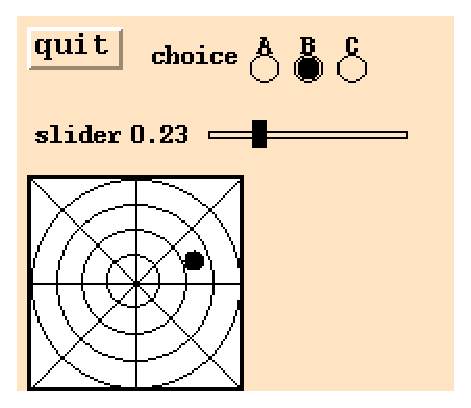
\includegraphics[height=5cm]{fig/panelitem.ps}
%\epsfile{file=fig/panelitem.ps,height=5cm}
%\mbox{
%\epsfysize=5cm
%\epsfbox{fig/panelitem.ps}
%}
\end{center}
\caption{Panel items created in a panel\label{panelitem}}
\end{figure}


\begin{refdesc}
\classdesc{text-item}{panel-item}
{(textwin)}{
{\tt Text-item} is used to display or to input one short line of text,
such as a file name.
A {\tt text-item} has a label string followed by
a small textwindow on the right.
When the pointer is put in the textwindow, key input is enabled
and the characters typed are buffered.
Line editing is available in the textwindow: 
{\tt control-F} and {\tt control-B} to move forward/backward by one character,
{\tt del} to delete the character on the left of the cursor,
{\tt control-D} to delete the character on the cursor, and
any graphical character to insert it at the cursor position.
Clicking a mouse button moves the cursor to the clicked character.
Hitting an enter (newline) key causes the buffered text to be sent to
the {\em notify-object}'s {\em notify-method}.}

\longdescription{:create}{label revciever method \= \&rest args \` [method]\\
\>\&key (font font-courb12) (columns 20) (initial-value ) (border-width 0)\\
\>\&allow-other-keys}{
creates text-item.
Though the linebuffer of the textwindow may have unlimited length,
visible portion is restricted to the {\em columns} characters.}

\methoddesc{:getstring}{}{
returns the string in the key buffer.}

%\methoddesc{:KeyPress}{pos}{
%if key is pressed, print key character to cursor position.}

%\methoddesc{:keyEnter}{ch}{
%prints {\em ch} to cursor position. But if {\em ch} is backspace,
%deletes 1 character from buffer. And if {\em ch} is return or newline,
%ignores.}
\end{refdesc}

\subsection{Canvas}
\begin{refdesc}
\classdesc{canvas}{xwindow}{(topleft bottomright)}{
Canvas is a xwindow to interact with figures or images.
Currently, only the region selection capability has been implemented.
At the buttonPress event, the canvas begins to draw a rectangle
with the topleft corner at the pressed position and bottomright corner
at the current pointer.
ButtonRelease causes the {\tt notify-method} to be sent to the {\tt notify-object}.
Use Xdrawable's methods to draw figures or images in the canvas.}

%\methoddesc{:adjust-corners}{}{
%corrects toleft and bottomright.}

%\methoddesc{:region-selection}{}{
%prints canvas region.}

%\methoddesc{:draw-selection-rectangle}{}{
%draws a rectangle that shows canvas region.}

%\methoddesc{:ButtonPress}{event}{
%reverses the color of button that shows {\em event}.}
%\methoddesc{:MotionNotify}{event}{
%makes selection rectangle which corners are pressed position 
%and cursor position.}
%\methoddesc{:ButtonRelease}{event}{
%clears selection rectangle and prints item on this canvas region.}

%\methoddesc{:clear-canvas}{item}{
%ignores {\em item}.}

\end{refdesc}

\subsection{Text Window}

There are three textwindow classes, {\tt TextWindow}, {\tt BufferTextWindow}
and {\tt ScrollTextWindow}.

\begin{refdesc}
\classdesc{textWindow}{xwindow}
{(fontid \\
\>charwidth charheight charascent dots \\
\>win-row-max win-col-max \\
\>win-row win-col \hspace{20mm} \= ;physical current position in window \\
\>x y\\
\>charbuf \>; for charcode conversion \\
\>keybuf keycount \> ;for key input\\
\>echo \\
\>show-cursor cursor-on \> ;boolean\\
\>kill delete \> ;control character \\
\>notify-object notify-method \\
\>)}{
realizes virtual terminals usable for displaying messages.
The displayed contents are not buffered and there is no way to retrieve
a line or a character already displayed in the TextWindow.
Basically, {\tt TextWindow} has similar capabilities to the dumb terminals,
that are, moving the cursor, erasing lines, erasing areas,
scrolling displayed texts, inserting strings, etc.
Also, the text cursor can be moved to the position designated by 
the mouse pointer.}

\methoddesc{:init}{id}{
initializes {\em id}th text-window.}

\longdescription{:create}{\=\&rest args \` [method]\\
\>\&key \=width height (font font-courb14) rows columns\\
\>(show-cursor nil) (notify-object nil) (notify-method nil)\\
\>\&allow-other-keys}{
creates text-window.
The sizes of the window may be specified either by {\em width} and {\em height}
or by {\em rows} and {\em columns}.
{\em Notify-object}'s {\em notify-method} is invoked when a newline character
is typed in.}

%\methoddesc{:set-notify}{reciever method}{
%}

\methoddesc{:cursor}{flag}{
The {\em flag} can either be {\tt :on, :off} or {\tt :toggle}.
The text cursor is addressed by the {\em win-row} and {\em win-col}. 
The text cursor is displayed if {\em flag} is {\tt :on},
is erased if {\em flag} is {\tt :off},
or is reversed if {\em flag} is {\tt :toggle}.
This method must be invoked frequently
whenever the character at the cursor is updated.}

\methoddesc{:clear}{}{
clears text-window.}

\methoddesc{:clear-eol}{\&optional (r win-row) (c win-col) (csr :on)}{
clears the rest of the line after the character
addressed by {\rm r} and {\em c}, including the character at the cursor.
}

\methoddesc{:clear-lines}{lines \&optional (r win-row)}{
clears multiple lines after {\em r}-th row.}

\methoddesc{:clear-eos}{\&optional (r win-row) (c win-col)}{
clears the region after the character addressed by {\em r} and {\em c}
till the end-of-the-screen.}

\methoddesc{:win-row-max}{}{returns the maximum number of lines
displayable in this window.}

\methoddesc{:win-col-max}{}{returns the maximum number of columns
displayable in this window.}

\methoddesc{:xy}{\&optional (r win-row) (c win-col)}{
calculates the pixel coordinates of the character 
addressed by {\em r} and {\em c}.}

\methoddesc{:goto}{r c \&optional (cursor :on)}{
moves the cursor to {\em r}-th row and {\em c}-th column.
}

\methoddesc{:goback}{\&optional (csr :on)}{
moves the cursor backward by one.}

\methoddesc{:advance}{\&optional (n 1)}{
moves the cursor forward by {\em n} characters.}

\methoddesc{:scroll}{\&optional (n 1)}{
scroll textwindow vertically by {\em n} lines.}

\methoddesc{:horizontal-scroll}{\&optional (n 1)}{
horizontally scrolls the text by {\em n} columns.}

\methoddesc{:newline}{}{
moves cursor to the beginning of the next line.}

\methoddesc{:putch}{ch}{
inserts the character {\em ch} at the cursor position.
The rest of the line is moved forward by one.}

%\methoddesc{:putstr}{str \&optional (e (length str))}{
%prints {\em str} to text-window.}
%
\methoddesc{:putstring}{str \&optional (e (length str))}{
places {\em str} at the cursor position.}

%\methoddesc{:getstring}{}{gets key-buffer.}

\methoddesc{:event-row}{event}{}
\methoddesc{:event-col}{event}{
returns the text cursor position designated by $(x, y)$ in the {\em event}.}
%\methoddesc{:EnterNotify}{event}{}
%\methoddesc{:ButtonPress}{event}{}
%\methoddesc{:ButtonRelease}{event}{}
%\methoddesc{:resize}{w h}{}
%\methoddesc{:ConfigureNotify}{event}{}
%\methoddesc{:keyrelease}{}{nob}
%\methoddesc{:enterNotify}{event}{}
%\methoddesc{:LeaveNotify}{event}{}
\methoddesc{:KeyPress}{event}{
inserts the character entered at the cursor position.
If the character is newline, notification is sent to the {\em notify-object}.}
%\methoddesc{:keyEnter}{ch}{}
%\methoddesc{:LineEnter}{ch}{}
%\methoddesc{:clear-text}{item}{clear text-window.}

\classdesc{textWindowStream}{stream}{(textwin)}{
{\tt TextWindowStream} is an output stream connected to a TextWindow.
Characters or strings output to this stream by using {\tt print, format,
write-byte}, etc., are displayed in the textwindow.
As usual file streams, the output data are buffered.}

\methoddesc{:flush}{}{
flushes buffered text string and send them to the textwindow.
{\tt Finish-output} or writing a newline character to this stream
automatically calls this method.}

\funcdesc{make-text-window-stream}{xwin}{
makes text-window-stream and returns the stream object.}

\classdesc{BufferTextWindow}{TextWindow}{
(linebuf expbuf max-line-length row col)}{
maintains the line buffer representing the contents of the textwindow.
Linebuf is the vector of lines. Expbuf holds tab-expanded text.
Only lines displayable in the window are maintained.
BufferTextWindows can be used as simple text editors
which have several, often only one, lines of text.
{\tt Text-item} employs a BufferTextWindow as a displayable line buffer.}

%\methoddesc{:create}{\&rest args}{}
%\methoddesc{:clear}{}{}
%\methoddesc{:goto}{r c \&optional (csr :on)}{}
\methoddesc{:line}{n}{returns the contents of the {\em n}-th line as a
string.}

\methoddesc{:nlines}{}{returns number of lines in the linebuf.}
\methoddesc{:all-lines}{}{returns the linebuf, which is a vector of strings.}
\methoddesc{:refresh-line}{\&optional (r win-row) (c win-col)}{
redraws the {\em r}-th line after the {\em c}-th column.}
\methoddesc{:refresh}{\&optional (start 0)}{
redraws the lines after the {\em start}-th line inclusively.}
\methoddesc{:insert-string}{string}{
inserts {\em string} at the cursor position.}
\methoddesc{:insert}{ch}{inserts the character at the cursor.}
\methoddesc{:delete}{n}{deletes {\em n} characters after the cursor.}
%\methoddesc{:keyEnter}{ch \&optional event}{}
%\methoddesc{:ButtonRelease}{event}{}

\funcdesc{expand-tab}{src \&optional (offset 0)}{
{\em Src} is a string possibly containing tabs.
These tabs are replaced by spaces assuming the tab stops at every 8th
position.}

\classdesc{ScrollTextWindow}{BufferTextWindow}{
(top-row top-col \hspace{30mm} \= ;display-starting position \\
\> scroll-bar-window \\
\> horizontal-scroll-bar-window \\
\> selected-line)}{
{\tt ScrollTextWindow} defines buffertextwindow with unlimited number of lines,
and vertical and horizontal scroll-bars can be attached.
ScrollTextWindow can handle {\tt :configureNotify} event to resize 
itself and accompanying scroll-bar windows, and to redisplay texts.
By clicking, a line can be selected.}

\methoddesc{:create}{\&rest args
           \&key (scroll-bar nil)
                (horizontal-scroll-bar nil)
           \&allow-other-keys}{
When scroll-bars are needed, specify T to each keyword argument.}

%\methoddesc{:locate-scroll-bar}{}{}
%\methoddesc{:clear}{}{}
%\methoddesc{:lines}{}{}
%\methoddesc{:max-line-length}{}{}
%\methoddesc{:refresh}{\&optional (offset 0) (lines (- win-row-max offset))}{}
%\methoddesc{:line-in-window-p}{ln}{}
%\methoddesc{:refresh-line}{ln \&optional (highlight nil) \&aux fg-save bg-save}{
%}
\methoddesc{:locate}{n}{displays the buffered text by placing the {\em n}-th
line at the top of the window.}
\methoddesc{:display-selection}{selection}{{\em Selection} represents
the location of the selected line. The entire seleced line is displayed
highlighted.}

\methoddesc{:selection}{}{returns the selected line (string).}

\methoddesc{:read-file}{fname}{reads the textfile specified by {\em fname}
into the {\em linebuf}, expands tabs, and display in the window.
The cursor is put at the beginning of the screen.}

\methoddesc{:display-string}{strings}{{\em Strings} is a sequence
of lines (strings). The {\em strings} are copied in the linebuf
and displayed in the window.}

%\methoddesc{:scroll-fraction}{}{}
%\methoddesc{:horizontal-scroll-fraction}{}{}

\methoddesc{:scroll}{n}{vertically scrolls {\em n} lines.}
\methoddesc{:horizontal-scroll}{n}{horizontally scrolls {\em n} columns.}
%\methoddesc{:insert-char}{c \&optional (refresh t)}{}
%\methoddesc{:insert-newline}{\&optional (refresh t)}{}
%\methoddesc{:insert}{thing \&optional (refresh t)}{}
%\methoddesc{:buttonPress}{event}{}
\methoddesc{:buttonRelease}{event}{
The line where the mouse pointer is located is selected.
If notification is specified when the window is created,
{\em notify-object}'s {\em notify-method} is invoked.}
\methoddesc{:resize}{w h}{changes the size of the window
and redisplays the contents according to the new size.
The same message is sent to scroll-bars if attached.}
%\methoddesc{:ConfigureNotify}{event}{}

%\classdesc{xitem}{xwindow}
%{(label labeldots width height)}{
%defines xitem that is used for pulldown menu.}

%\methoddesc{:draw-label}{}{
%draws xitem's label.}

%\longdescription{:create}{label \= \&rest args \hspace{120mm} [method]\\
%\>\&key width height (font font-cour10)\\
%\>\&allow-other-keys}{
%creates xitem.}

% \classdesc{input-panel}{panel}{}{
% defines input-lines for panel. Input-panel is a one line input window that
% has quit button, cancel button and input line with under-line. 
% This class is used by xinput function.}
% 
% \methoddesc{:getstring}{}{
% gets key-buffer.}
% 
% \methoddesc{:quit}{\&rest args}{
% quit this input line window.}
% 
% \methoddesc{:input-line}{\&rest args}{
% quit this input line window.}
% 
% \methoddesc{:create}{title len \&rest args}{
% creates input line window. And add 'CANCEL' button on this window.}
% 
%\funcdesc{xitem-length}{label \&key (font font-cour10)}{
%returns {\em label}'s length.}

%\funcdesc{xset-eachground}{win fg bg \&optional (f-flag t)}{
%sets {\em win}'s foreground color and background color. And {\em win} refresh.
%But if {\em f-flag} is nil, {\em win} don't refresh.}

% \funcdesc{x::xinput}{\&key (title "Input:") (len 30) (font font-cour10) (par *root*) x y}{
% creates input-panel positioned ({\em x},{\em y}), then gets string. 
% If input is end, returns input string, and destroys this input-panel. 
% When input string is nothing, returns nil. Notes that mouse cursor have
% to be moved on the input area, whenever you input text.}

\end{refdesc}

\newpage
